\section{Prototype implementation}

In this section we provide a detailed description of our framework and the technologies that are used in the front and back ends, the data collection and last the different aspects of data visualization.


\subsection{Framework}

Our web application is based on Django\footnote{\url{https://www.djangoproject.com/}}, which is a free and open-source web framework, written in Python, and follows the model–view–controller (MVC) architectural pattern. We used HTML, CSS and JavaScript in the front-end and Python, JavaScript in the back-end. First, the application is using the retrieved data for politicians and athletes from JSON files for all the tasks that will be performed. Then, the application analyzes the data further for visualizing different aspects of user contributions. For producing the dynamic, interactive data visualizations we use the JavaScript library D3.
The application provides an overview of that data with different visualizations for presenting the user contribution over the time, users summary of posts, impact of posts and the topics that a user is discussing.


\subsection{Data Collection}

Our data collection consists of real-world data from Facebook 
and Twitter and focus on 28 public persons such as, politicians 
and athletes because they tend to post the same content on Twitter and Facebook more than a normal user. The attributes of the data along with their definitions are displayed in Table \ref{table:attrib_des}. The below data was saved in different files for each user in JSON format.

\begin{table}[ht] 
\caption{Description of the attributes of data} 
\centering  
\begin{tabular}{c | c} 
\hline\hline 
Attribute & Description \\ [0.5ex] 
\hline 
ID & The id of the post \\ 
date & The date of the post \\ 
text & The text of the post\\ 
likes & The number of likes of a post \\ [1ex]  
\hline  
\end{tabular} 
\label{table:attrib_des}
\end{table}

\subsubsection{Retrieve data from Facebook}
The data from Facebook was obtained by using the Facebook Graph API with the Facebook JavaScript SDK. First, we got all the posts for one user by using his username and saved them in a database. After obtaining all the posts we called the API again with the post-id of each post to get a summary of all the likes,which we also saved in a database.

\subsubsection{Retrieve data from Twitter}

The data was obtained by quering the timeline API of Twitter with the username of each person related to politicians and athletes. For this procedure we used  Tweepy\footnote{\url{http://www.tweepy.org/}}, which is a Python library for accessing the Twitter API. We were able to collect a fixed number of tweets because Twitter only allows access to a users most recent 3240 tweets.  

\subsection{Back-end}
Before we could visualize the data, we had to analyze it and convert it to a format which could be put in a visualization. We used Python as a programming language to process the data. For the calculation of the topic models or similarities of posts we used a library called scikit-learn\footnote{\url{http://scikit-learn.org}}, a free software machine learning library.   

\subsection{Data visualization}
The data visualization was done using the JavaScript library D3\footnote{\url{https://d3js.org/}}, which produces dynamic and interactive data visualizations for the web. Embedded in an HTML webpage, one can create SVG objects, customize them, add data bindings and transitions  with the D3 library. A big advantage of JavaScript D3 is that, there exist many examples using the library, which makes it easier to learn it and produce nice visualizations. \\
In the following paragraphs we want to illustrate which layouts and diagrams of the library we used to visualize our data. 


\subsubsection{Contribution over time}
We decided to show the contribution over time in a monthly interval. Therefore, we calculated how many posts a user wrote in each month in each social network. 
After this we used a matrix diagram to visualize the contributions. Each row in the matrix corresponds to a year and social network and each column corresponds to a month. Consequently, the value of a cell displays the contribution of a user in a month of a specific year in one social network. Instead of writing the real value in the cell, we used circles to visualize the amount of contribution. The number of posts where mapped to a range of $0$ to $20$, which then where used as the radius of the circles. Hence, the size of a circle was the greatest when the most posts were published in this time. 


In Figure \ref{fig:contribution} one can see an example of this approach. In this diagram we showed the contribution over time for Barack Obama. As already mentioned in section \ref{sec:uservisualization}, a visualization like this one can help to identify the month where important events happened. If we would analyze the graphic we probably would say that the November in 2011 was an important month for Barack Obama, as he posted there many more than in the other months. If a user of our prototype is interested in the posts of November 2011, he can click on the corresponding circle and the program shows all posts of this month at the side. Figure \ref{fig:contribution2} shows, how this looks like.  

\begin{figure}[t]
	\centering
	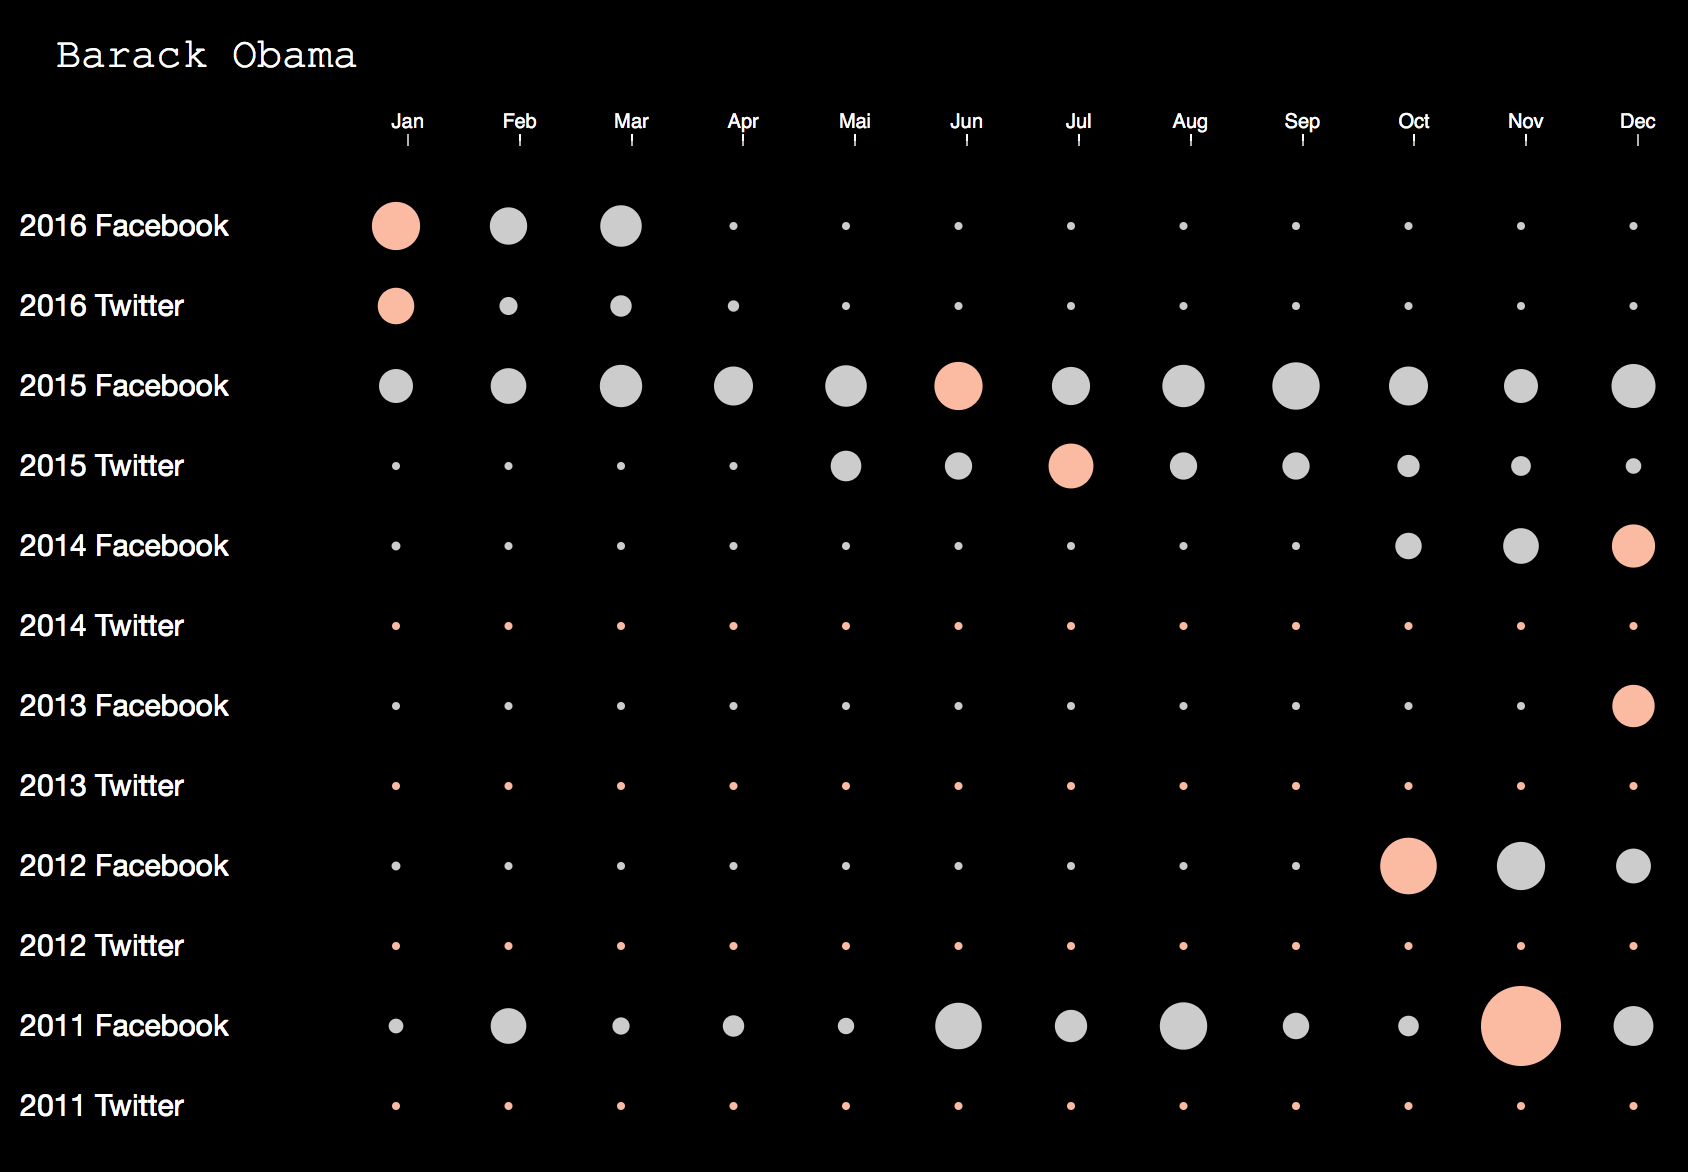
\includegraphics[width=0.7\linewidth]{usercontribution}
	\caption{Example contribution over time for Barack Obama}
	\label{fig:contribution}
\end{figure}

\begin{figure}[t]
	\centering
	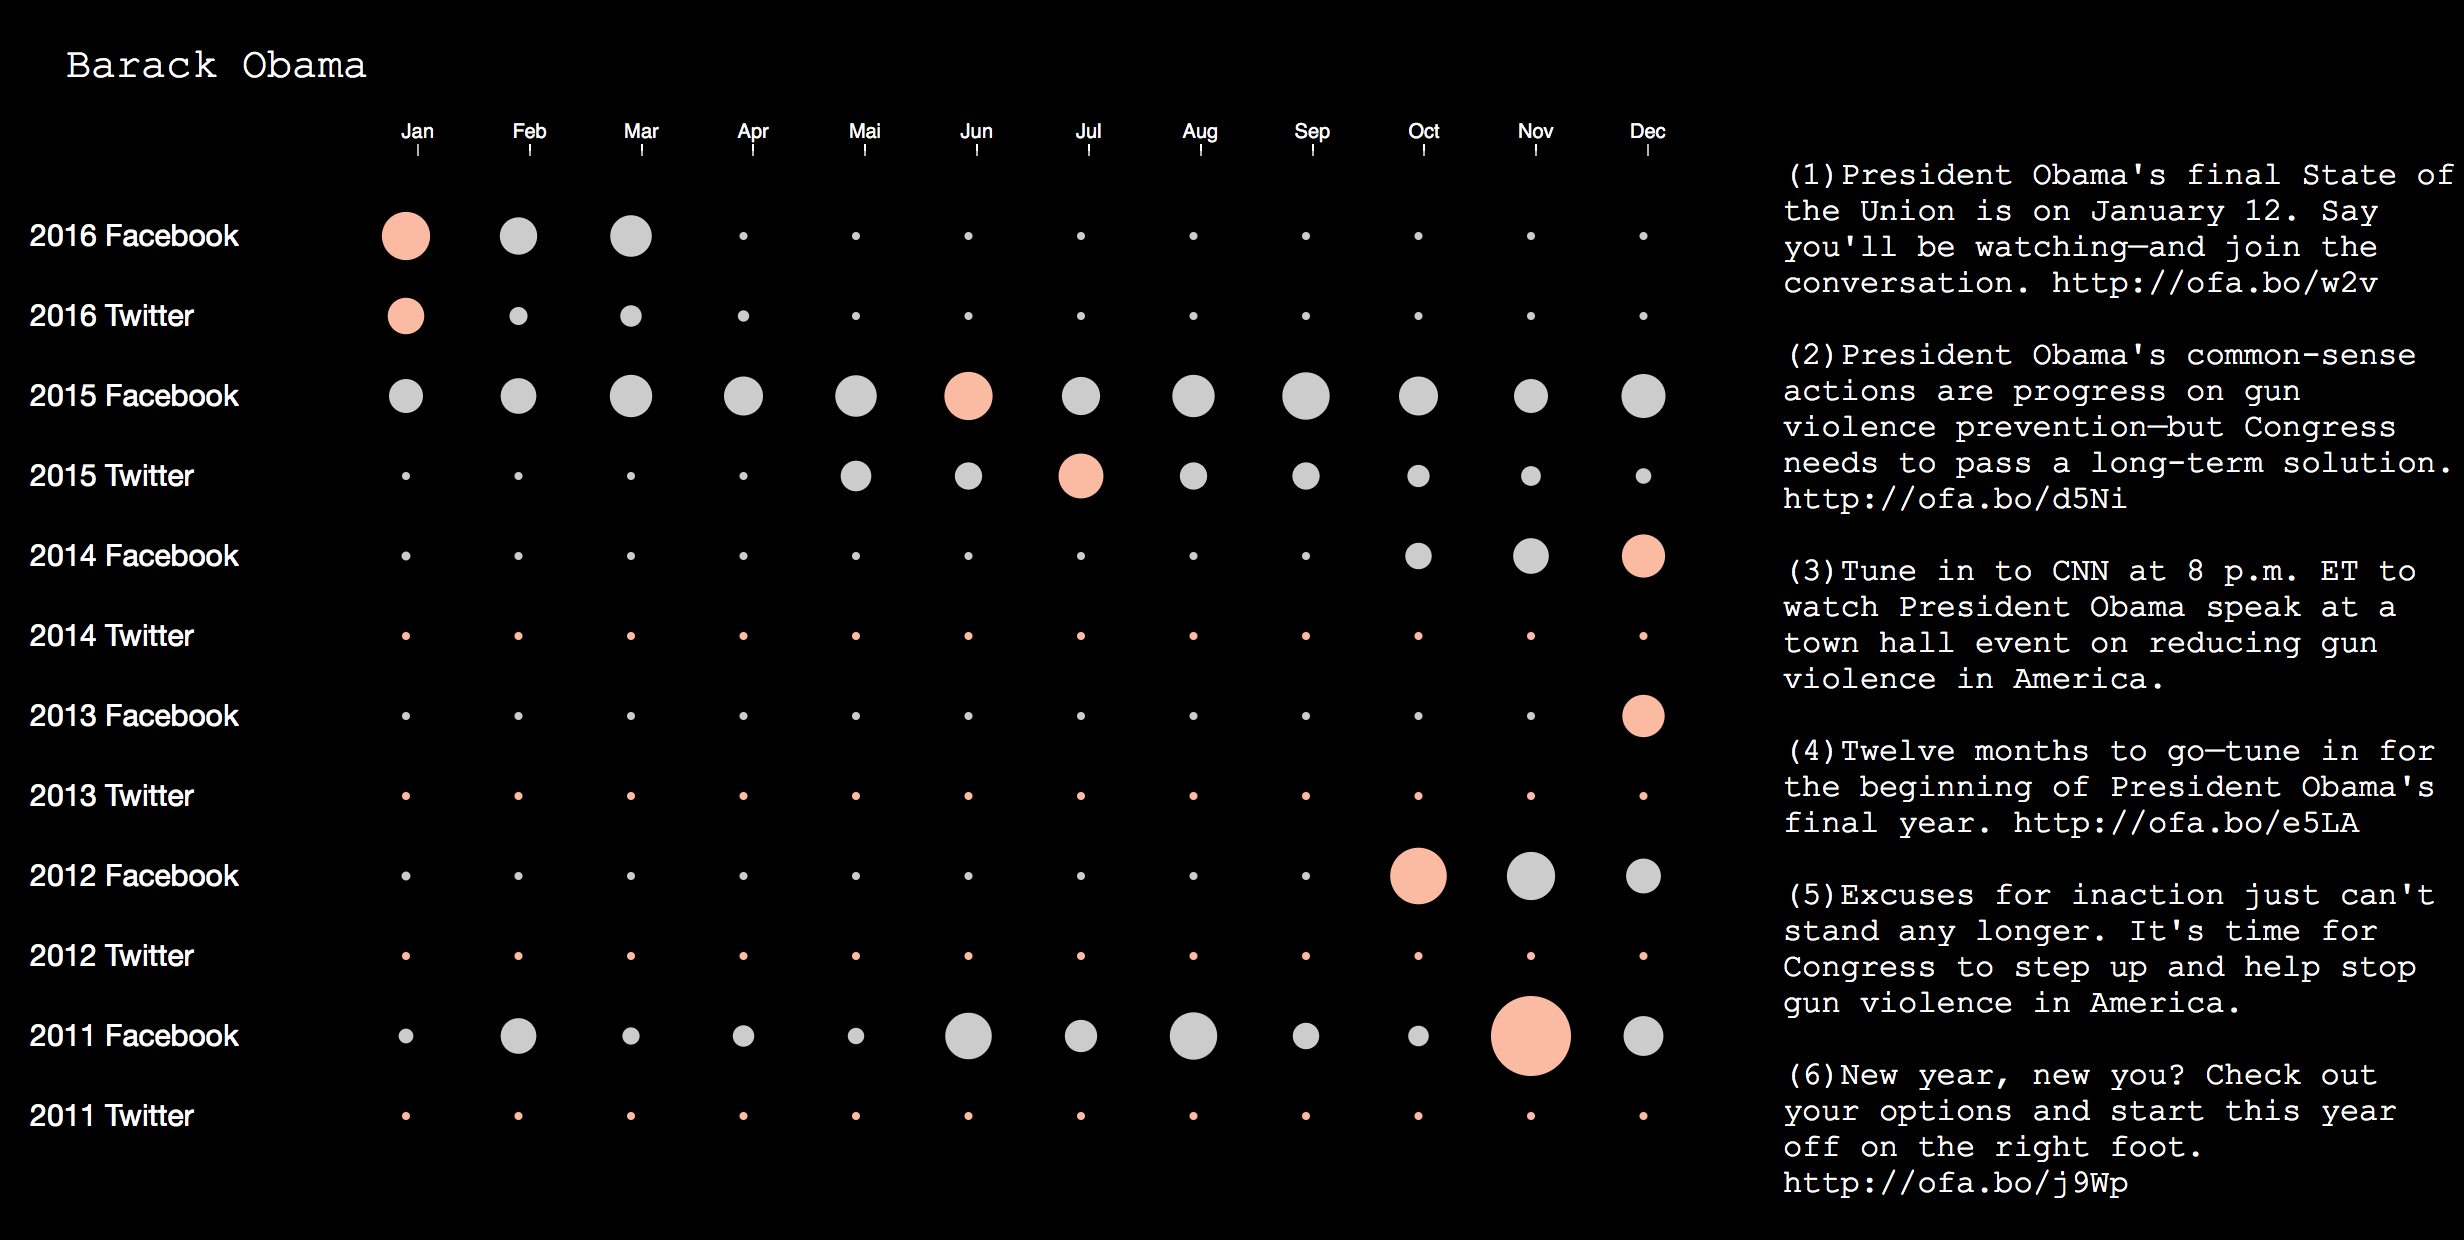
\includegraphics[width=0.7\linewidth]{usercontribution1}
	\caption{Example contribution over time for Barack Obama with post showing}
	\label{fig:contribution2}
\end{figure}

\subsubsection{Summary of posts}


For visualizing a summary of the posts, we used the approach shown in section \ref{sec:graphVisualization}. To recap, this approach gives us a graph, where each distinct word of our corpus is represented as a node and each co-occurring words are connected by an edge. Each node has a occurrence-count based on how often the word is used and each edge has a weight based on how often the connected words co-occur together.


Before visualizing the posts, a user can choose a time range, this can be a month in a year or the last X days. The algorithm then, just visualizes the summary of all the posts, which were published in this time range.


After getting the posts and calculating the graph, the structure is drawn. We used the Force Layout from the JavaScript D3 library, because it takes automatically care that, strongly connected components are close to each other, while components which are not strongly connected are further away from each other. This results in a better overview of the data. 


The size of a label of a node was adjusted to the occurrence-count of this node. This means that the more often a word occurs in the text, the bigger the size of the label of the corresponding node. For the edges we did something similar. As more often two words appear together, as thicker we draw the connection between the corresponding nodes.


In  Figure \ref{fig:summary}, one can see an example of our approach. We visualize the summary of the posts of Barack Obama of January 2016 by considering the $25$ most used words. As we can see, the more connected components around "Barack", "President" and "Obama" are closer to each other, than the other nodes, which make it easier to read the structure. For further information a user of our prototype can go over one edge with his mouse which opens a text box with all the posts in which the two corresponding word co-occurred together. An example of this is shown in Figure \ref{fig:summary2}.

\begin{figure}[t]
	\centering
	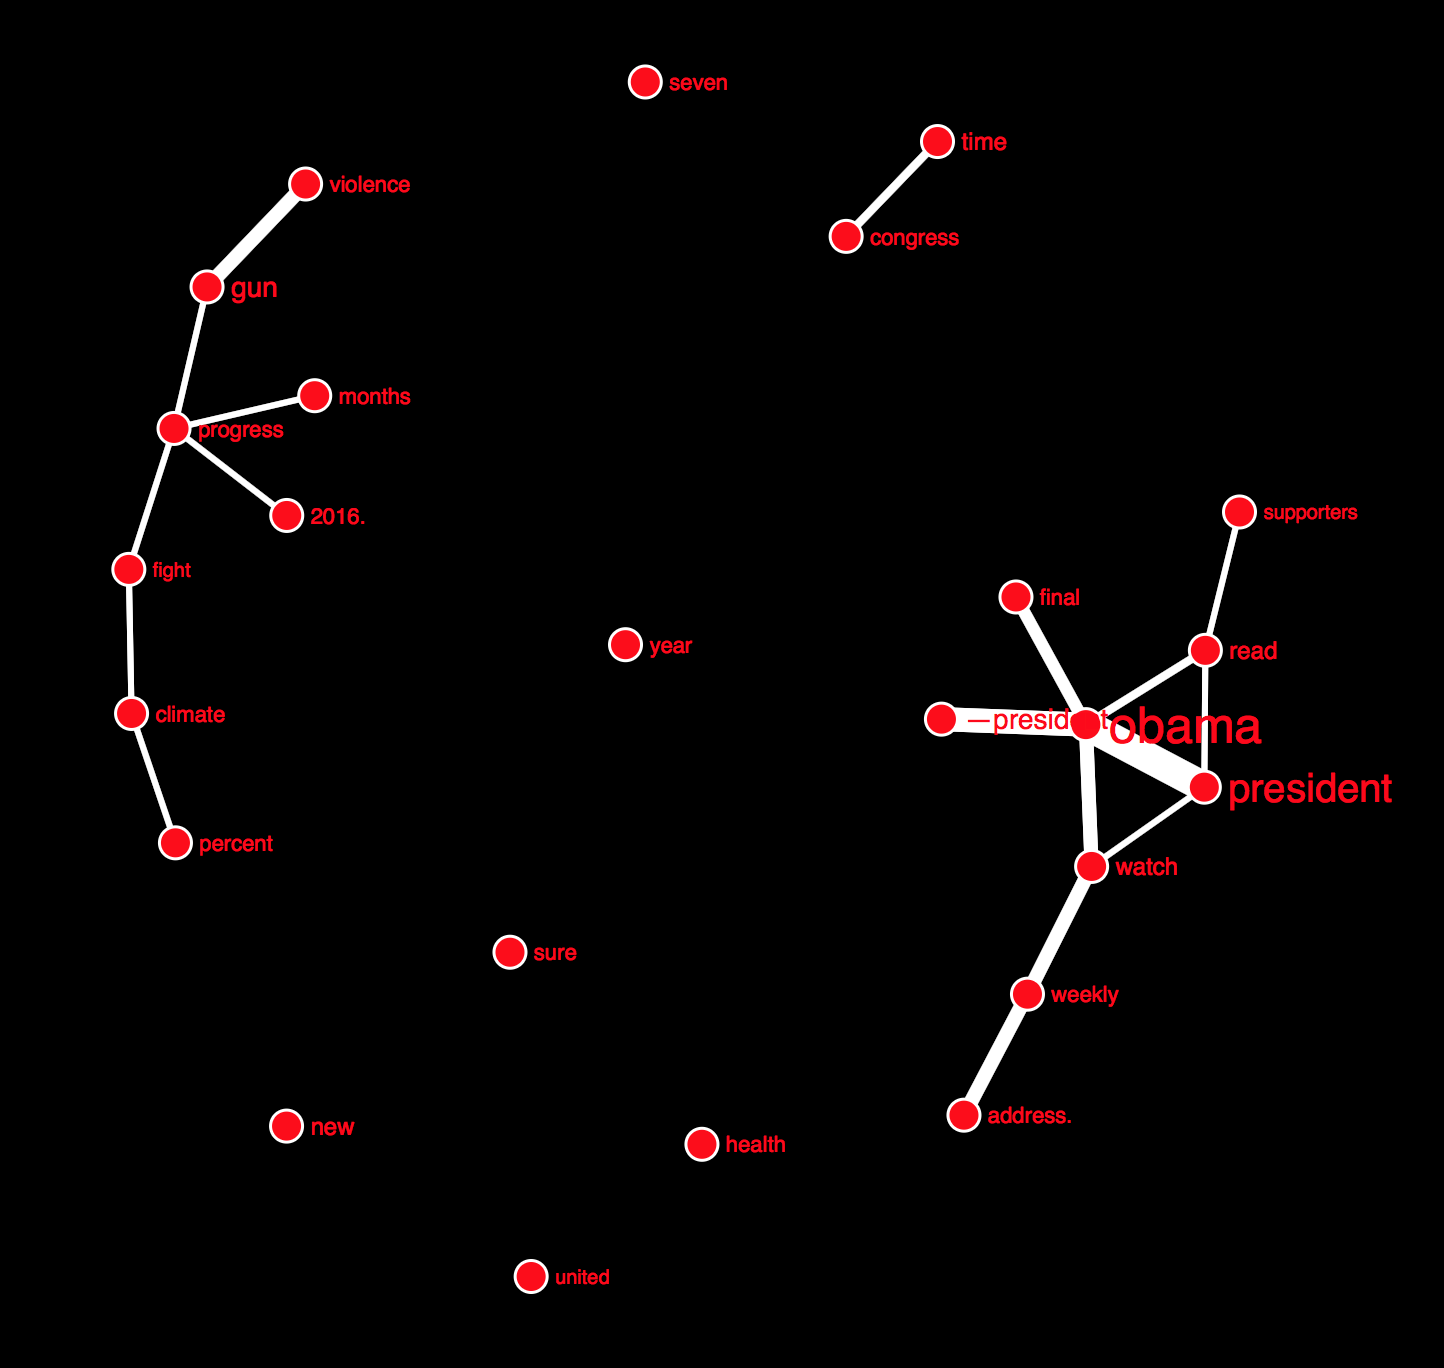
\includegraphics[width=0.7\linewidth]{summary1}
	\caption{Example of the summary of posts of Barack Obama of January 2016}
	\label{fig:summary}
\end{figure}


\begin{figure}[t]
	\centering
	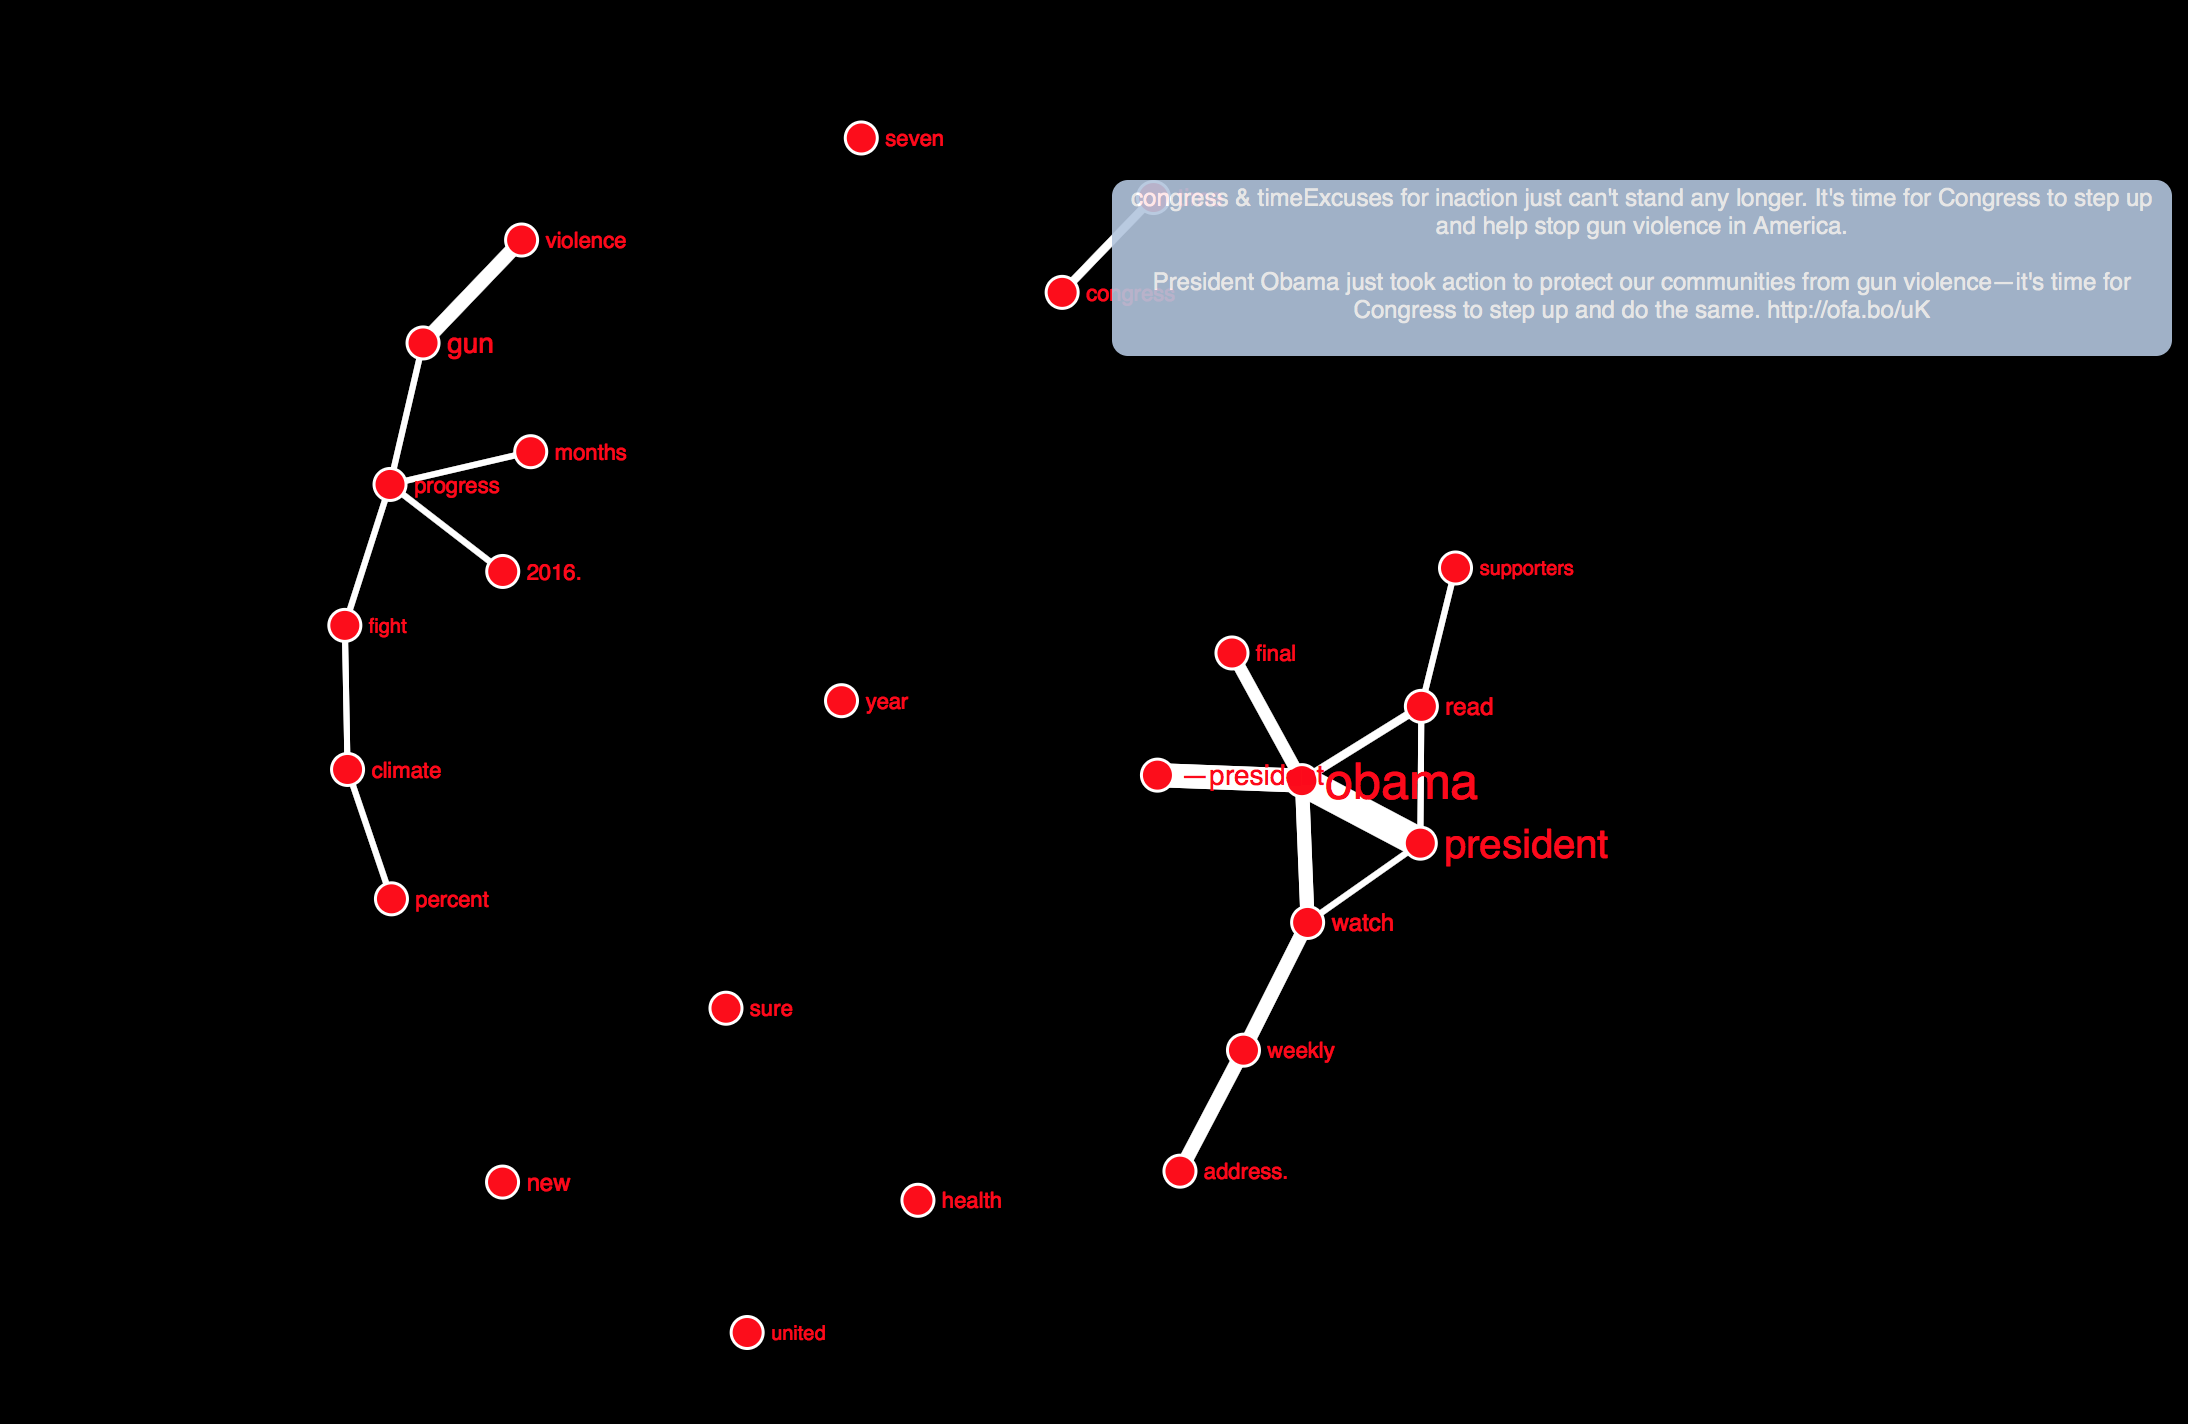
\includegraphics[width=0.7\linewidth]{summary2}
	\caption{Example of the summary of posts with mouse-over of Barack Obama of January 2016}
	\label{fig:summary2}
\end{figure}


\subsubsection{Topic models}


For calculating the topic models we used the "LatentDirichletAllocation" class from the scikit-learn library. When initializing an object of this class, one has to  decide how many topics should be created. A method called "fit" calculates these topic models and returns for each topic model a ranked list of words, which are used to describe the topic. We also used a method called  "transform" which returns 
a document-topic matrix, where a cell $ c_{i,j} $ indicates how probable the document i belongs to the topic j. With this matrix, we assigned to each document the most probable topic, which gave us an overview about which document belongs to which topic and how many documents a topic has.  


An example for a part of the  output of the "fit" method can be seen in table \ref{tab:exampleOutputTopicModels}. Here, we calculated 5 topic models for the posts of Barack Obama.


For the visualization of the models we wanted to show the top $5$ words for each topic to the user, as well as, how many documents belong to each topic. While, the top $5$ words give us a description of the models, the visualization of the amount of documents for each topics gives us an impression about how important each topic is. It is assumed that, a topic which has many more documents than the other topics, is more important to the writer than another topic.


We chose a Bubble Chart from the D3 library to realize our ideas. In the chart we assigned each topic a bubble (circle), which size is depending on how many documents belong to this topic. Inside the chart we wrote the top 5 words, to describe the model. Figure \ref{fig:chart} shows an example of this approach. Here we created 10 topics for the post of Barack Obama. The number of topics to be calculated can be chosen by the user of our framework. For further information a user can go with his mouse over one topic and see the number of documents which belong to this topic, as well as other words, which describe this topic (Figure \ref{fig:chart2}). If the user clicks on one of the bubbles, the documents (post) of this topic are shown at the side. This approach enables a user to find out what a person is talking about, as well as just getting the posts about the topics the user is actually interested in. 

\begin{table}
	\centering
	\begin{tabular}{c|c|c|c|c|c}

&  word 1 & word  2 & word  3 & word   4 & word  5 \\ 
\hline
Topic \quad1 & house & president &  white &  obama &  barack \\ 
\hline
Topic \quad2 & president  & change  & obama  & climata  & people  \\ 
\hline
Topic \quad3 & president & obama  & reform  &  day  & court  \\ 
\hline
Topic \quad4 & 2012   &  check  &  deal & love  &  iran \\ 
\hline
Topic \quad5 &  obama & president  & watch   & america  &  day
\end{tabular}
\caption{Example output for LDA Topic Models}\label{tab:exampleOutputTopicModels}
\end{table}


\begin{figure}[t]
	\centering
	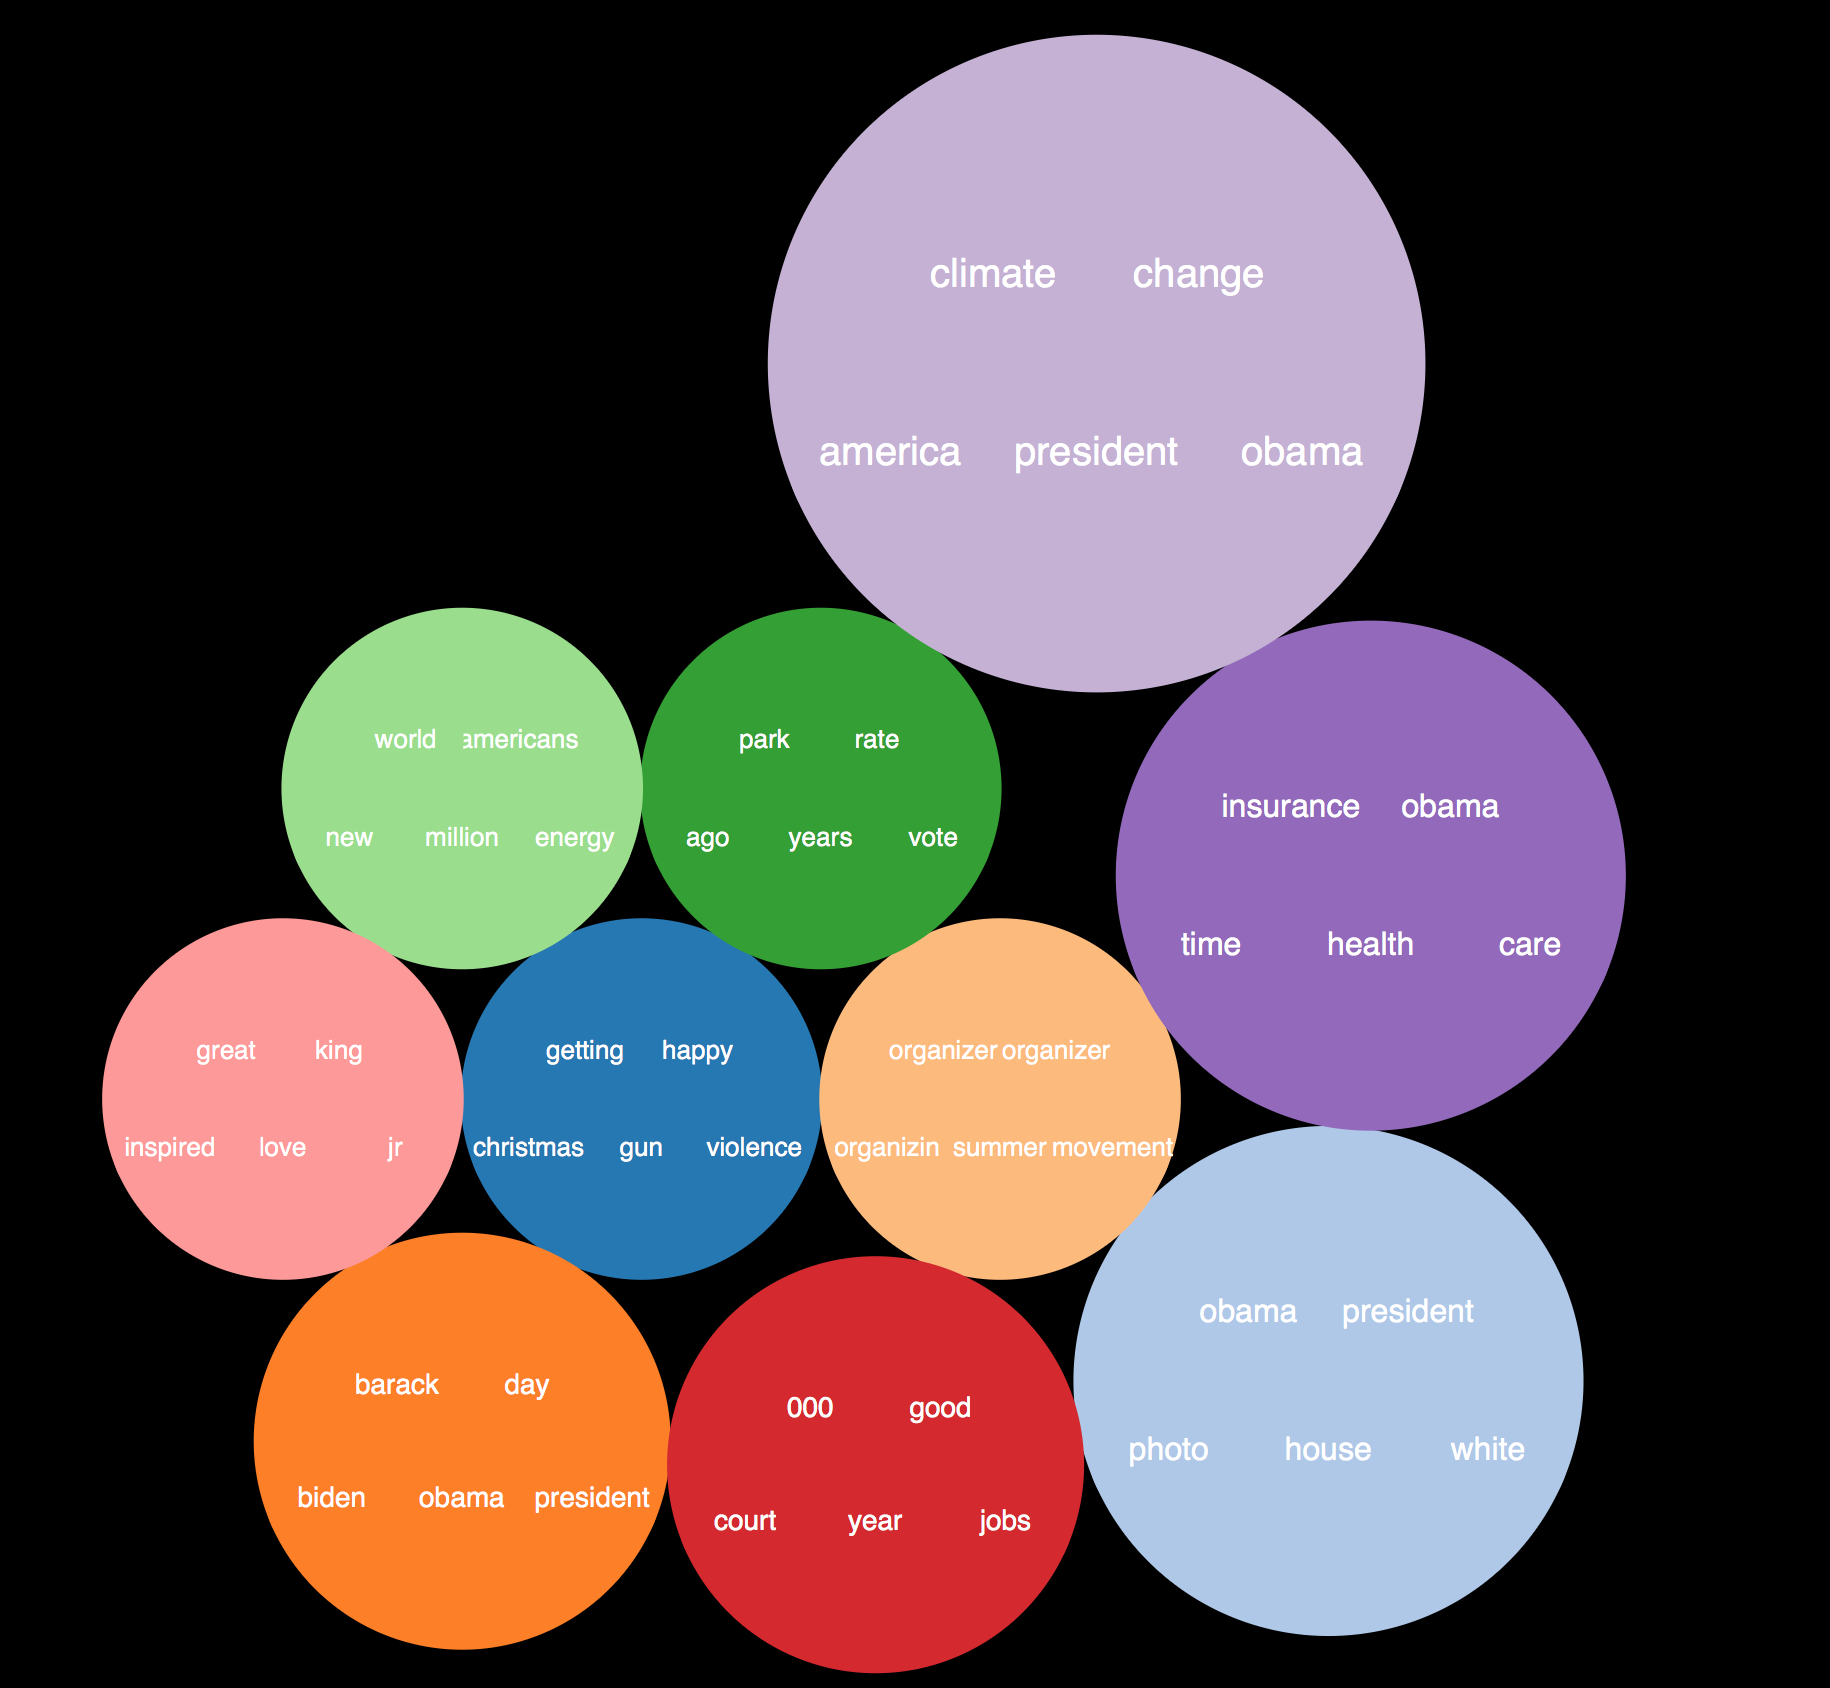
\includegraphics[width=0.7\linewidth]{topicModel}
	\caption{Topic model examples for Barack Obama}
	\label{fig:chart}
\end{figure}


\begin{figure}[t]
	\centering
	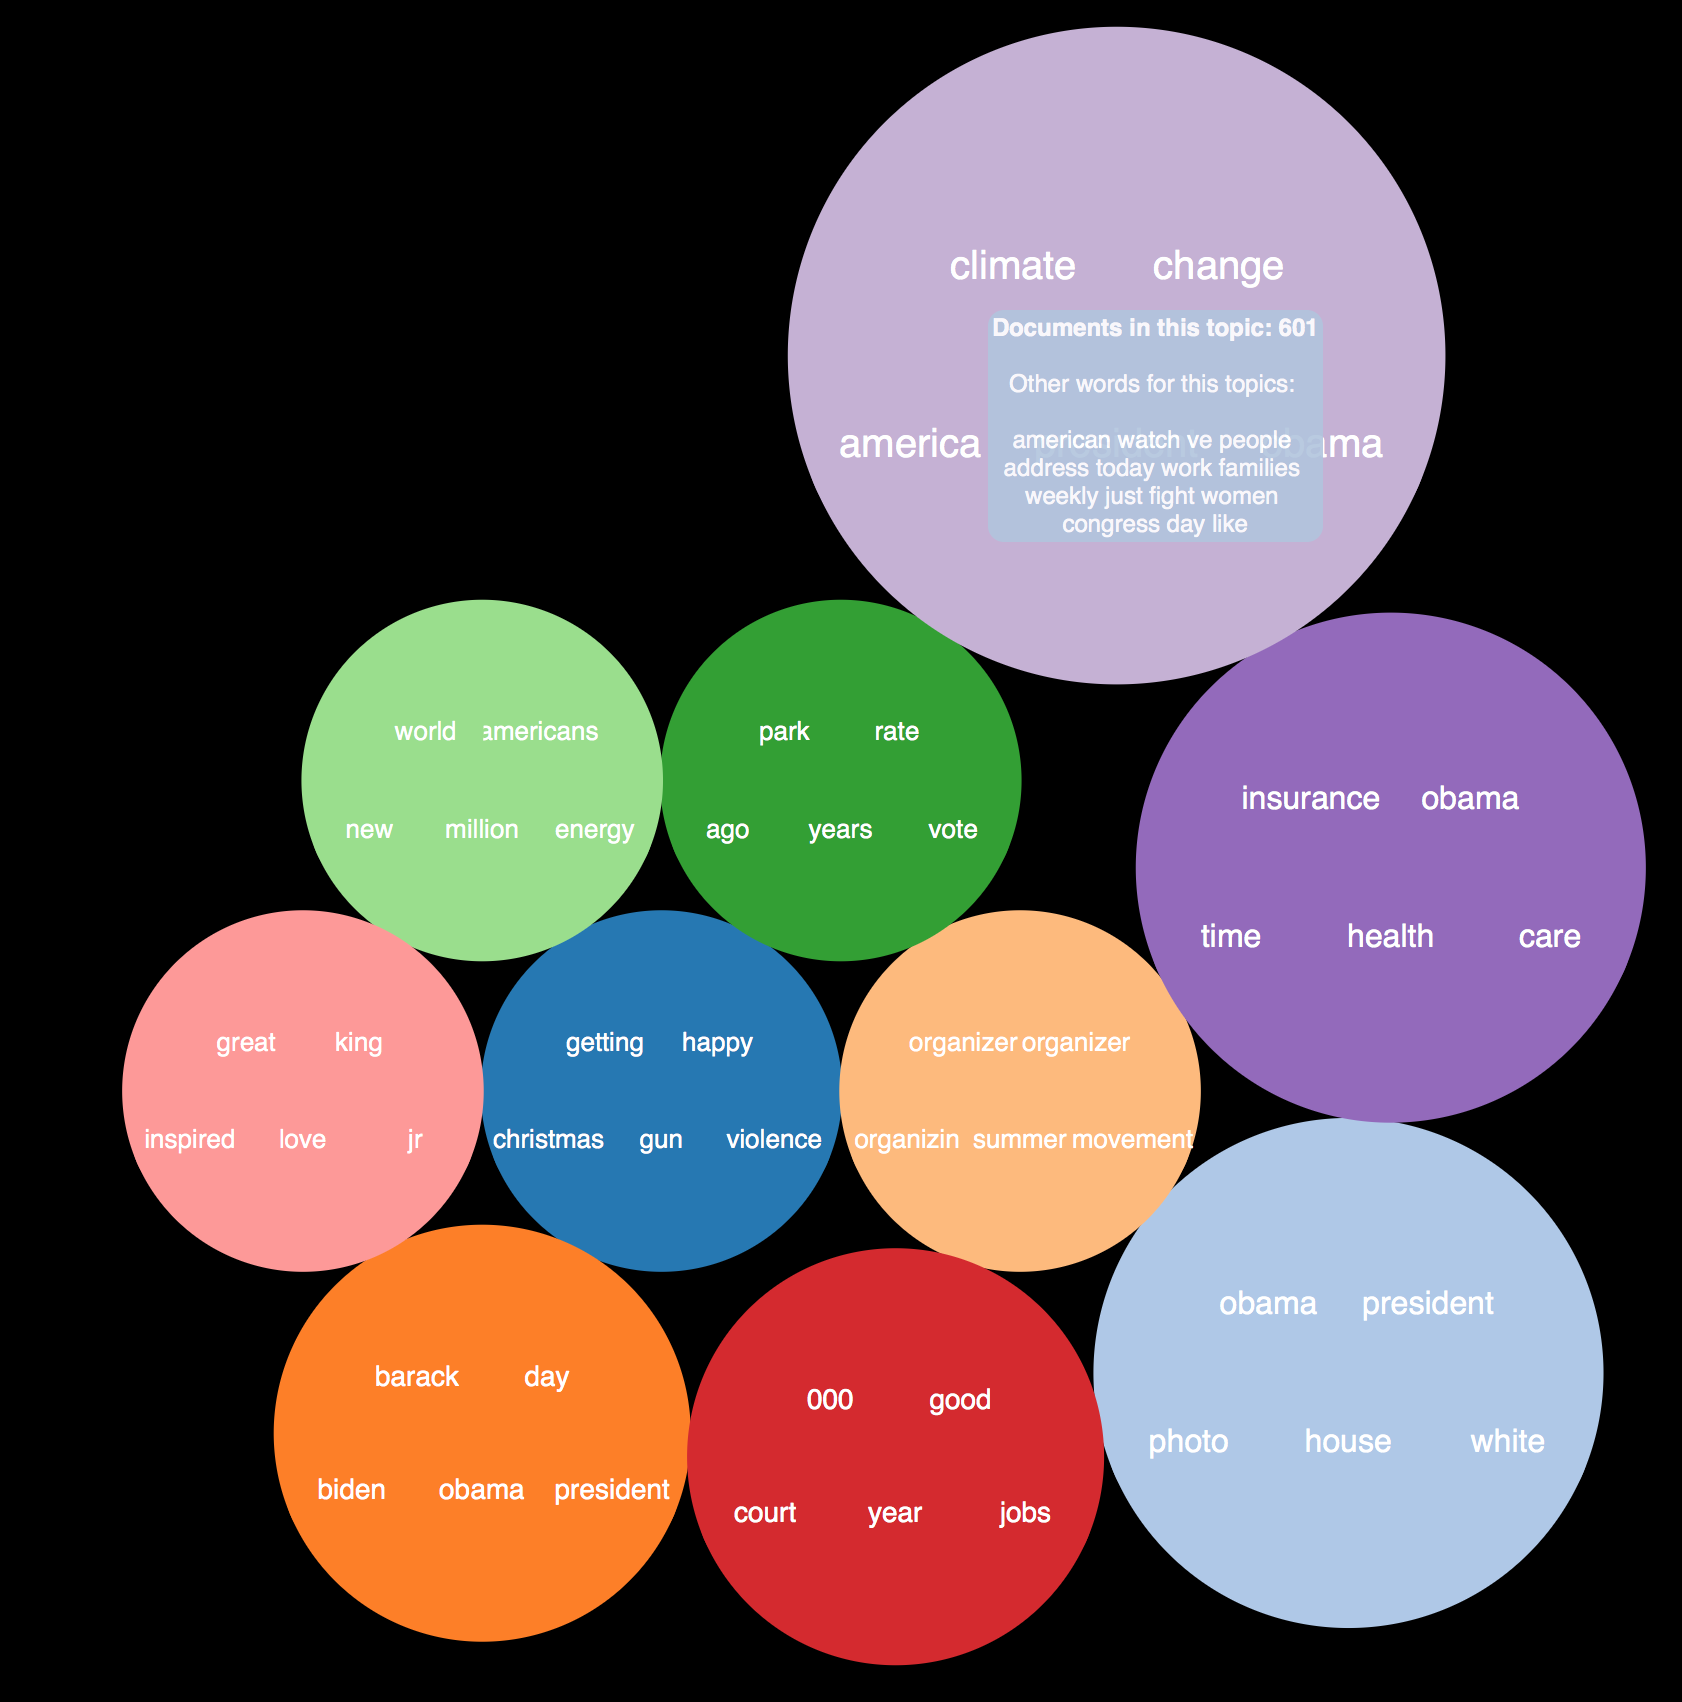
\includegraphics[width=0.7\linewidth]{topicModel2}
	\caption{Topic model examples with mouse-over for Barack Obama}
	\label{fig:chart2}
\end{figure}


\subsubsection{Impact of posts}


To compare the impact a post has in different social networks, we had to first find similar post from one person in the different social networks. We used the following algorithm to accomplish this task: 

\begin{algorithm}
 \scriptsize
	\SetKwInOut{Input}{Input}
	\SetKwInOut{Output}{Output}
	
	\Input{Collection X of posts from Facebook and collection Y of post from Twitter}
	\Output{The most similar post in Twitter for each  Facebook post}
	\ForEach {post x in X}
	{
		init maximum\_similarity = 0
		init most\_similar\_post = None
		\ForEach  {post y in Y}
		{
			calculate cosine similarity between x and y
			\If {similarity  > maximum\_similarity}
			{
				maximum\_similarity = similarity
				most\_similar\_post = y
			}
		}
		
	}				
	\caption{Algorithm to find the most similar Twitter post for a Facebook post}
\end{algorithm}

We predefined a threshold to accept two similar posts if they have a similarity of at least $60\%$. This portion lets us a great amount of similar posts and also recognize twitter posts that have urls, hashtags and mentions.

\begin{figure}[t]
	\centering
	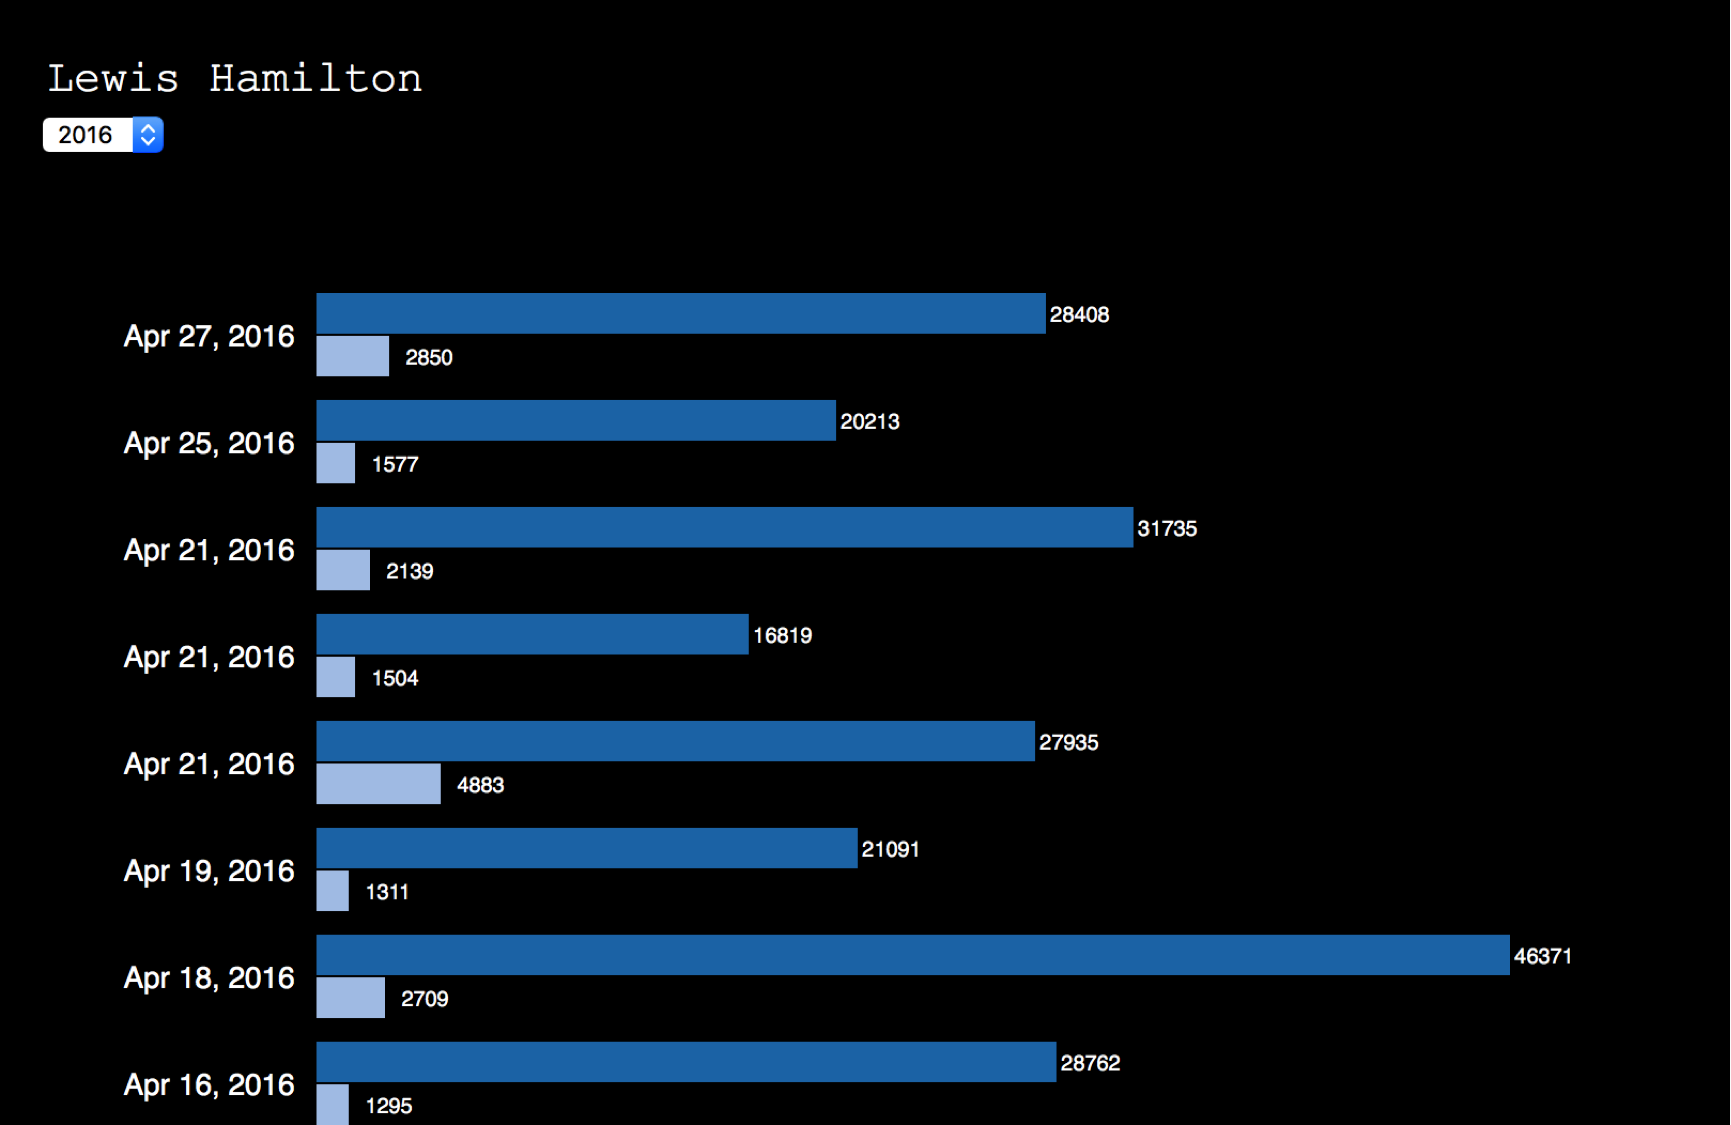
\includegraphics[width=0.7\linewidth]{timeline}
	\caption{The impact of posts written by Lewis Hamilton.}
	\label{fig:impact}
\end{figure}

The visualization was then done with a vertical Bar Chart. We created a timeline which showed the date on which two similar post were published and one bar for the number of likes for the post in its social network. With this chart, a user of our framework gets an information about the number of likes of each post which were published on Facebook and Twitter and can compare these numbers. Figure \ref{fig:impact} shows an example of this visualization. In this figure we show the impact of post written by Lewis Hamilton. To find out the content of the post a user can just go over one bar with the mouse and the content is displayed. 




%%% Local Variables: 
%%% mode: latex
%%% TeX-master: "isae-report-template"
%%% End: 